\chapter{System infrastructure: wake, sleep, memory를 어떻게 잇는가}
\label{STC-S13}

세 개의 logical plane이 곧 세 개의 physical cluster를 뜻하지 않는다. 필요한 것은 latency-critical wake
execution, throughput-oriented candidate construction, transactional publication의 책임 분리다. Load와
state locality가 허용하면 같은 accelerator pool을 time-partition할 수 있고, contention 또는 privacy가
크면 분리할 수 있다. 배치는 brain analogy가 아니라 bytes, queue, SLO 측정으로 결정한다.

\section{세 plane과 하나의 publication transaction}

\begin{enumerate}
  \item \textbf{Wake plane}: inference, retrieval, optional fast learning, event append를 latency SLO 안에서
  수행하고, 하나의 authorized serving head를 pin한다.
  \item \textbf{Sleep plane}: immutable wake snapshot을 읽어 extract, compact, graph update, replay,
  distill, adapter tune, policy update, rebuild, verify job을 수행한다. 결과는 candidate일 뿐 live state가
  아니다.
  \item \textbf{Memory/control plane}: raw evidence와 derived views의 lineage, version, authorization,
  capacity, atomic publish, rollback을 관리한다.
\end{enumerate}

Sleep transaction은 다음처럼 표현할 수 있다.

\begin{equation}
T(X_v,M_v,B,P)\rightarrow \widehat M_{v+1}
\xrightarrow[\text{compare-and-swap}]{\text{validate}} M_{v+1}.
\label{eq:sleep-transaction}
\end{equation}

$X_v$는 immutable event range, $M_v$는 published manifest, $B$는 resource budget, $P$는 frozen policy다.
Candidate는 old/new/safety/delete/poison/system canary를 통과한 뒤에만 manifest-last로 publish된다.
Reader는 요청 중 한 version을 보며 partial vector/metadata/adapter state를 섞어 보지 않는다.

\section{Source-of-record와 heterogeneous materialized views}

Derived memory의 governance basis로는 updated weights 하나보다 external source-of-record와 provenance
graph가 강하다.\claim{STC-C046}\autocite{srcstc0053,srcstc0063,srcstc0066} Raw event도 retention
policy가 허용하는 동안만 canonical이다. Text summary, vector, graph, latent/KV, adapter, shared weight는
모두 source lineage를 가진 materialized view로 취급한다.

\begin{table}[htbp]
\centering
\caption{Memory medium별 serving path와 rollback contract}
\label{tab:medium-contract}
\begin{tabularx}{\textwidth}{L{0.18\textwidth} L{0.20\textwidth} Y L{0.24\textwidth}}
\toprule
Medium & Wake path & Update/validation & Rollback basis \\
\midrule
raw episode & selective retrieval & append, redact, expire & event/version log \\
semantic text & prompt injection & rewrite, faithfulness & source span + predecessor \\
vector/graph & ANN/traversal & re-embed, edge validity & index generation + episode \\
latent/recurrent & accelerator state read & compatibility, semantic probe & checkpoint or source rebuild \\
adapter/expert & model forward/router & train, merge, old/new canary & base digest + delta version \\
shared weight & model forward & full regression/unlearning & checkpoint + training lineage \\
\bottomrule
\end{tabularx}
\end{table}

삭제는 tombstone 한 번이 아니다. Immediate access deny, online artifact invalidation, derived lineage rebuild,
backup/key expiry, behavioral residual test를 서로 다른 deadline으로 기록한다. Old checkpoint 전체를 되살리는
rollback은 그 사이의 delete/consent epoch를 되돌릴 수 있으므로, authorized sub-root만 새 generation으로
재조합해야 한다.

\section{Scheduler: operator, destination, cadence를 분리한다}

하나의 evidence region에 대한 action space는 NO\_OP, RETAIN\_EXACT, EXPIRE, DEDUP, MERGE,
ABSTRACT, GRAPH\_UPDATE, LATENT\_COMPILE, ADAPTER\_COMPILE, PARAMETRIC\_PROMOTE, DEMOTE,
REBUILD, QUARANTINE를 포함한다. Learned policy가 action을 제안해도 privacy, tenant boundary,
capacity, deadline, promotion gate는 hard constraint로 남긴다.

Batching key는 base model/tokenizer와 adapter shape, embedding/index version, privacy zone, deadline,
operator, source shard다. 같은 batch가 효율적이라는 이유로 tenant security domain을 합치지 않는다.
Preemption은 uncommitted candidate를 버릴 수 있어야 하고, wake saturation 시 sleep보다 wake가 우선한다.

Sleep service는 scalar FLOP queue가 아니라 resource vector queue다.

\begin{equation}
\mathbf c_j=(c_{GPU\text{-}s},c_{CPU\text{-}s},c_{HBM\text{-}byte\text{-}s},
c_{RAM\text{-}byte\text{-}s},c_{IO\text{-}byte},c_{net\text{-}byte}).
\end{equation}

Mean GPU utilization이 낮아도 source affinity, validation model, index lock, network link 때문에 P99 job age가
발산할 수 있다. Queue 안정성은 utilization 한 숫자뿐 아니라 privacy deadline과 tenant starvation으로
판정한다.

\section{State migration roofline}

Separate sleep cluster는 training accelerator utilization을 높일 수 있지만 source episode, base model,
optimizer, adapter candidate, validation trace를 이동시킨다. Link $\ell$마다 이동 bytes $B_\ell$, transfer
price/energy $p_\ell$, delay $T_\ell$, delay value $v_{delay}$를 두면

\begin{equation}
C_{move}=\sum_{\ell}\left(B_\ell p_\ell+T_\ell v_{delay}\right).
\end{equation}

추가 local execution과 replication cost가 $C_{move}$보다 작을 때만 compute를 data 쪽으로 옮긴다.
Model/optimizer residency가 source보다 훨씬 크면 centralized GPU가, source-to-delta ratio와 privacy locality가
크면 shard-local preprocessing이 유리할 수 있다.

\begin{figure}[htbp]
  \centering
  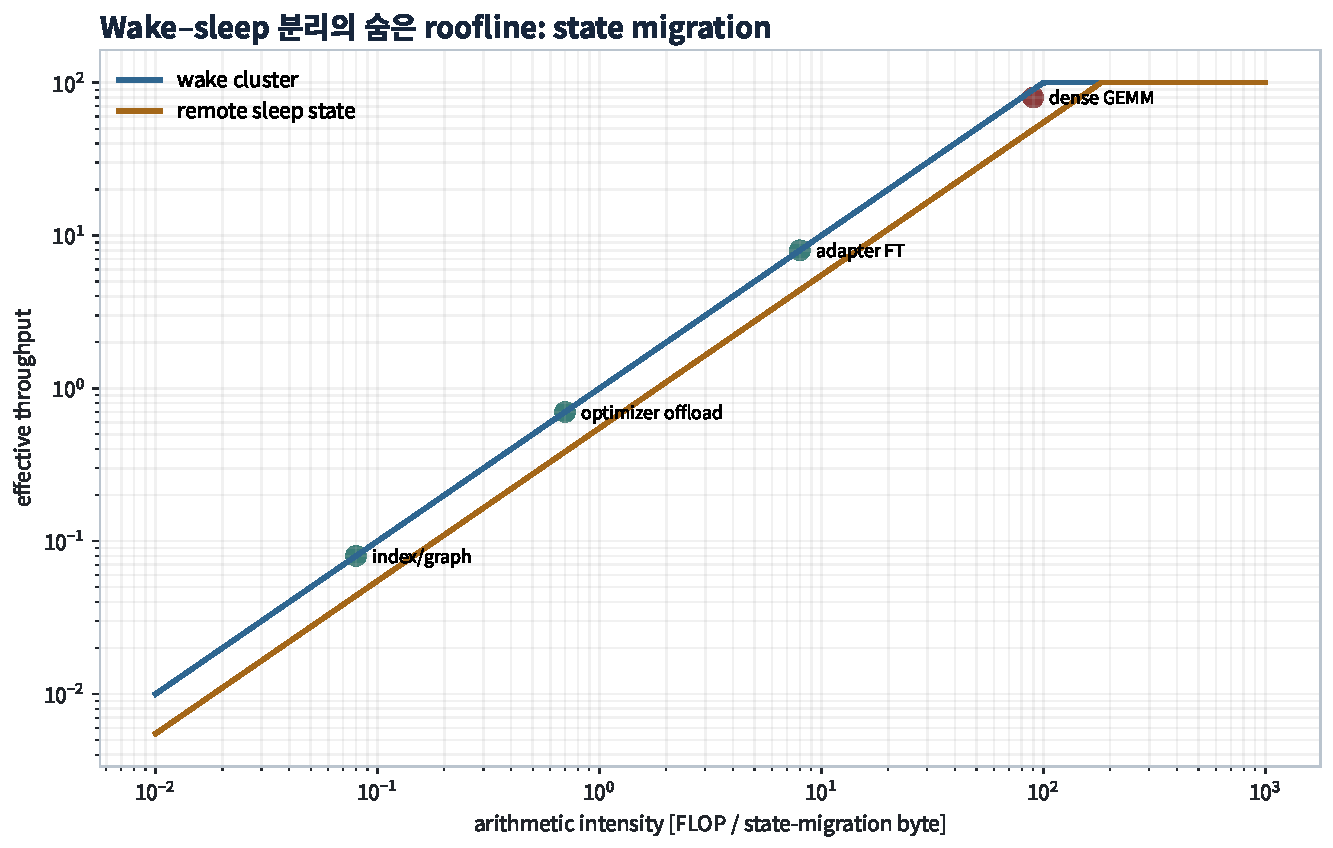
\includegraphics[width=0.97\textwidth]{figures/stc-f011.pdf}
  \caption{Wake/sleep placement의 state-migration roofline. Arithmetic intensity가 아니라 유용한 sleep
  work 대비 이동 state의 비율과 link bandwidth가 placement crossover를 정한다. 표시된 영역은 설계
  공간이며 특정 GPU의 측정 결과가 아니다.}
  \stcfigure{STC-F011}
  \figsource{Original systems synthesis; SRC-STC-0022, SRC-STC-0059}{Shared, separate, shard-local 배치를 state movement와 compute efficiency 축에서 비교한 roofline형 지도.}
  \label{fig:state-migration-roofline}
\end{figure}

\section{네 가지 physical placement}

\begin{longtable}{L{0.18\textwidth} L{0.22\textwidth} L{0.24\textwidth} L{0.21\textwidth}}
\caption{Physical placement option과 측정해야 할 trade-off}\label{tab:placement-options}\\
\toprule
Placement & 장점 & 비용/위험 & 적합 조건 \\
\midrule
\endfirsthead
\toprule
Placement & 장점 & 비용/위험 & 적합 조건 \\
\midrule
\endhead
shared priority fleet & base/model copy 최소, pooling & wake tail contention & sleep가 작고 preemptible \\
time-partitioned fleet & idle window 활용 & burst와 timezone mismatch & predictable diurnal load \\
separate wake/sleep & isolation, training batch 효율 & base replica와 network movement & sustained sleep demand \\
regional/shard-local hybrid & source locality, privacy & 낮은 local compute efficiency, fragmentation & source-to-delta ratio가 큼 \\
\bottomrule
\end{longtable}

\section{운영 계약}

Minimum viable system은 (1) append-only event log, (2) exact snapshot, (3) copy-on-write candidate,
(4) signed validation result, (5) atomic serving-head swap, (6) delete epoch와 deny root, (7) version-pinned
read, (8) bounded rollback과 GC owner를 가져야 한다. Algorithm quality가 좋아도 이 계약이 없으면 wake
request가 half-published state를 읽고, deleted source가 predecessor에서 부활하며, sleep retry가 duplicate
update를 만들 수 있다.

\begin{keypoint}[Infra 결론]
필요한 분리는 cluster의 개수가 아니라 responsibility와 transaction boundary다. Wake는 응답과 event
capture, sleep은 candidate construction, memory/control은 authoritative lineage와 publication을 담당한다.
Data 이동을 최소화한다는 말은 source만 보는 것이 아니라 base, optimizer, candidate, validation,
predecessor까지 같은 timestamp와 link에서 계측한다는 뜻이다.
\end{keypoint}
